\documentclass[letterpaper,11pt]{article}
\usepackage[utf8x]{inputenc}
\usepackage{enumerate}
\usepackage{fullpage}
\usepackage{amsmath}

\usepackage{pgf}
\usepackage{tikz}
\usetikzlibrary{arrows,shapes,trees}

%opening
\title{Physics 601 (Fall 2011) \\ Homework Assignment 2}
\date{Due: Thursday September 8, 2011}

\begin{document}

\maketitle

\paragraph*{Generalized Coordinates and the Lagrange's Equations}
\begin{itemize}
 \item If $L(\vec{q},\dot{\vec{q}},t)$ is a Lagrangian for a system of $n$ degrees of freedom satisfying Lagrange's equations, show that
  \begin{equation*}
   L'(\vec{q},\dot{\vec{q}},t) = L(\vec{q},\dot{\vec{q}},t) + \frac{dF}{dt}
  \end{equation*}
 also satisfies Lagrange's equations where $F(\vec{q},t)$ is any arbitrary, but differentiable, function of its arguments.
 \item A particle of charge $e$ in an electromagnetic field sees a generalized potential $U(\vec{r},\vec{v},t) = e \phi - e \vec{v} \cdot \vec{A}$.  Show that under the gauge transformation
  \begin{eqnarray*}
   \vec{A'} & = & \vec{A} + \vec{\nabla} \psi(\vec{r},t) \\
   \phi'    & = & \phi - \frac{\partial\psi(\vec{r},t)}{\partial t}
  \end{eqnarray*}
 the Lagrangian changes in a way consistent with the previous problem.
 \item A block of mass $m$ slides without friction down a wedge of mass $M$, which is free to slide without friction on a horizontal table.
 \begin{enumerate}
  \item Determine the Lagrangian for the system, using $q_1$ and $q_2$ as generalized coordinates.
  \item Determine the equations of motion.
  \item Let $\ell$ be the length of the sloping face of the wedge.  How long does it take the block to reach the table, assuming the entire system starts from rest with $q_1 = 0$?
 \end{enumerate}
 \textit{Note: This problem was part of the qualifying exam in August 2011.}
 \begin{center}
  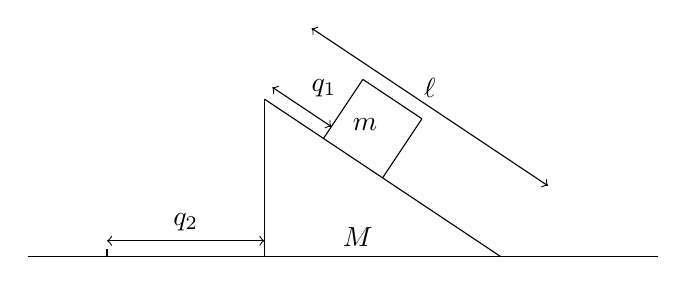
\begin{tikzpicture}
   % X axis
   \draw (-4,-0) -- (4,-0);
   \draw (-3,-0) -- (-3,0.1);
   % Wedge
   \draw (-1,0) -- (-1,2);
   \draw (-1,2) -- (2,0);
   \draw (-1,0) -- node[above left]{$M$} (2,0);
   \draw[<->] (-0.4,2.9) -- node[above]{$\ell$} (2.6,0.9);
   \draw[<->] (-3,0.2) -- node[above]{$q_2$} (-1,0.2);
   % Block
   \draw (-0.25,1.5) -- node[below right]{$m$} (0.25,2.25);
   \draw (0.25,2.25) -- (1,1.75);
   \draw (0.5,1) -- (1,1.75);
   \draw[<->] (-0.9,2.15) -- node[above right]{$q_1$} (-0.15,1.65);
  \end{tikzpicture}
 \end{center}
\end{itemize}

\end{document}
